\documentclass[a4paper,12pt]{article} 

%%% Работа с русским языком
\usepackage{cmap}                           % поиск в PDF
\usepackage{mathtext} 			 	       % русские буквы в формулах
\usepackage[T2A]{fontenc}               % кодировка
\usepackage[utf8]{inputenc}              % кодировка исходного текста
\usepackage[english,russian]{babel}  % локализация и переносы


\usepackage{wrapfig}


%Матеша
\usepackage{amsmath,amsfonts,amssymb,amsthm,mathtools} % AMS
\usepackage{icomma} % "Умная" запятая

%\mathtoolsset{showonlyrefs=true} % Показывать номера только у тех формул, на которые есть \eqref{} в тексте.

%% Шрифты
\usepackage{euscript}	 % Шрифт Евклид
\usepackage{mathrsfs} % Красивый матшрифт

%% Свои команды
\DeclareMathOperator{\sgn}{\mathop{sgn}}

%% Перенос знаков в формулах (по Львовскому)
\newcommand*{\hm}[1]{#1\nobreak\discretionary{}
{\hbox{$\mathsurround=0pt #1$}}{}}



%%% Заголовок
\author{Злобина Вера Б02-002}
\title{Лабораторная работа 2.2.1

Исследование взаимной диффузии газов}
\date{\today}

\begin{document}
	
\maketitle 
	
	
\newpage


\subparagraph*{Цель работы:}1)  регистрация  зависимости  концентрации   гелия в воздухе от времени с помощью датчиков теплопроводности при разных начальных давлениях смеси газов; 2) определение коэффициента диффузии по результатам измерений.

\begin{wrapfigure}{l}{0.30\linewidth} 
	\centering 
	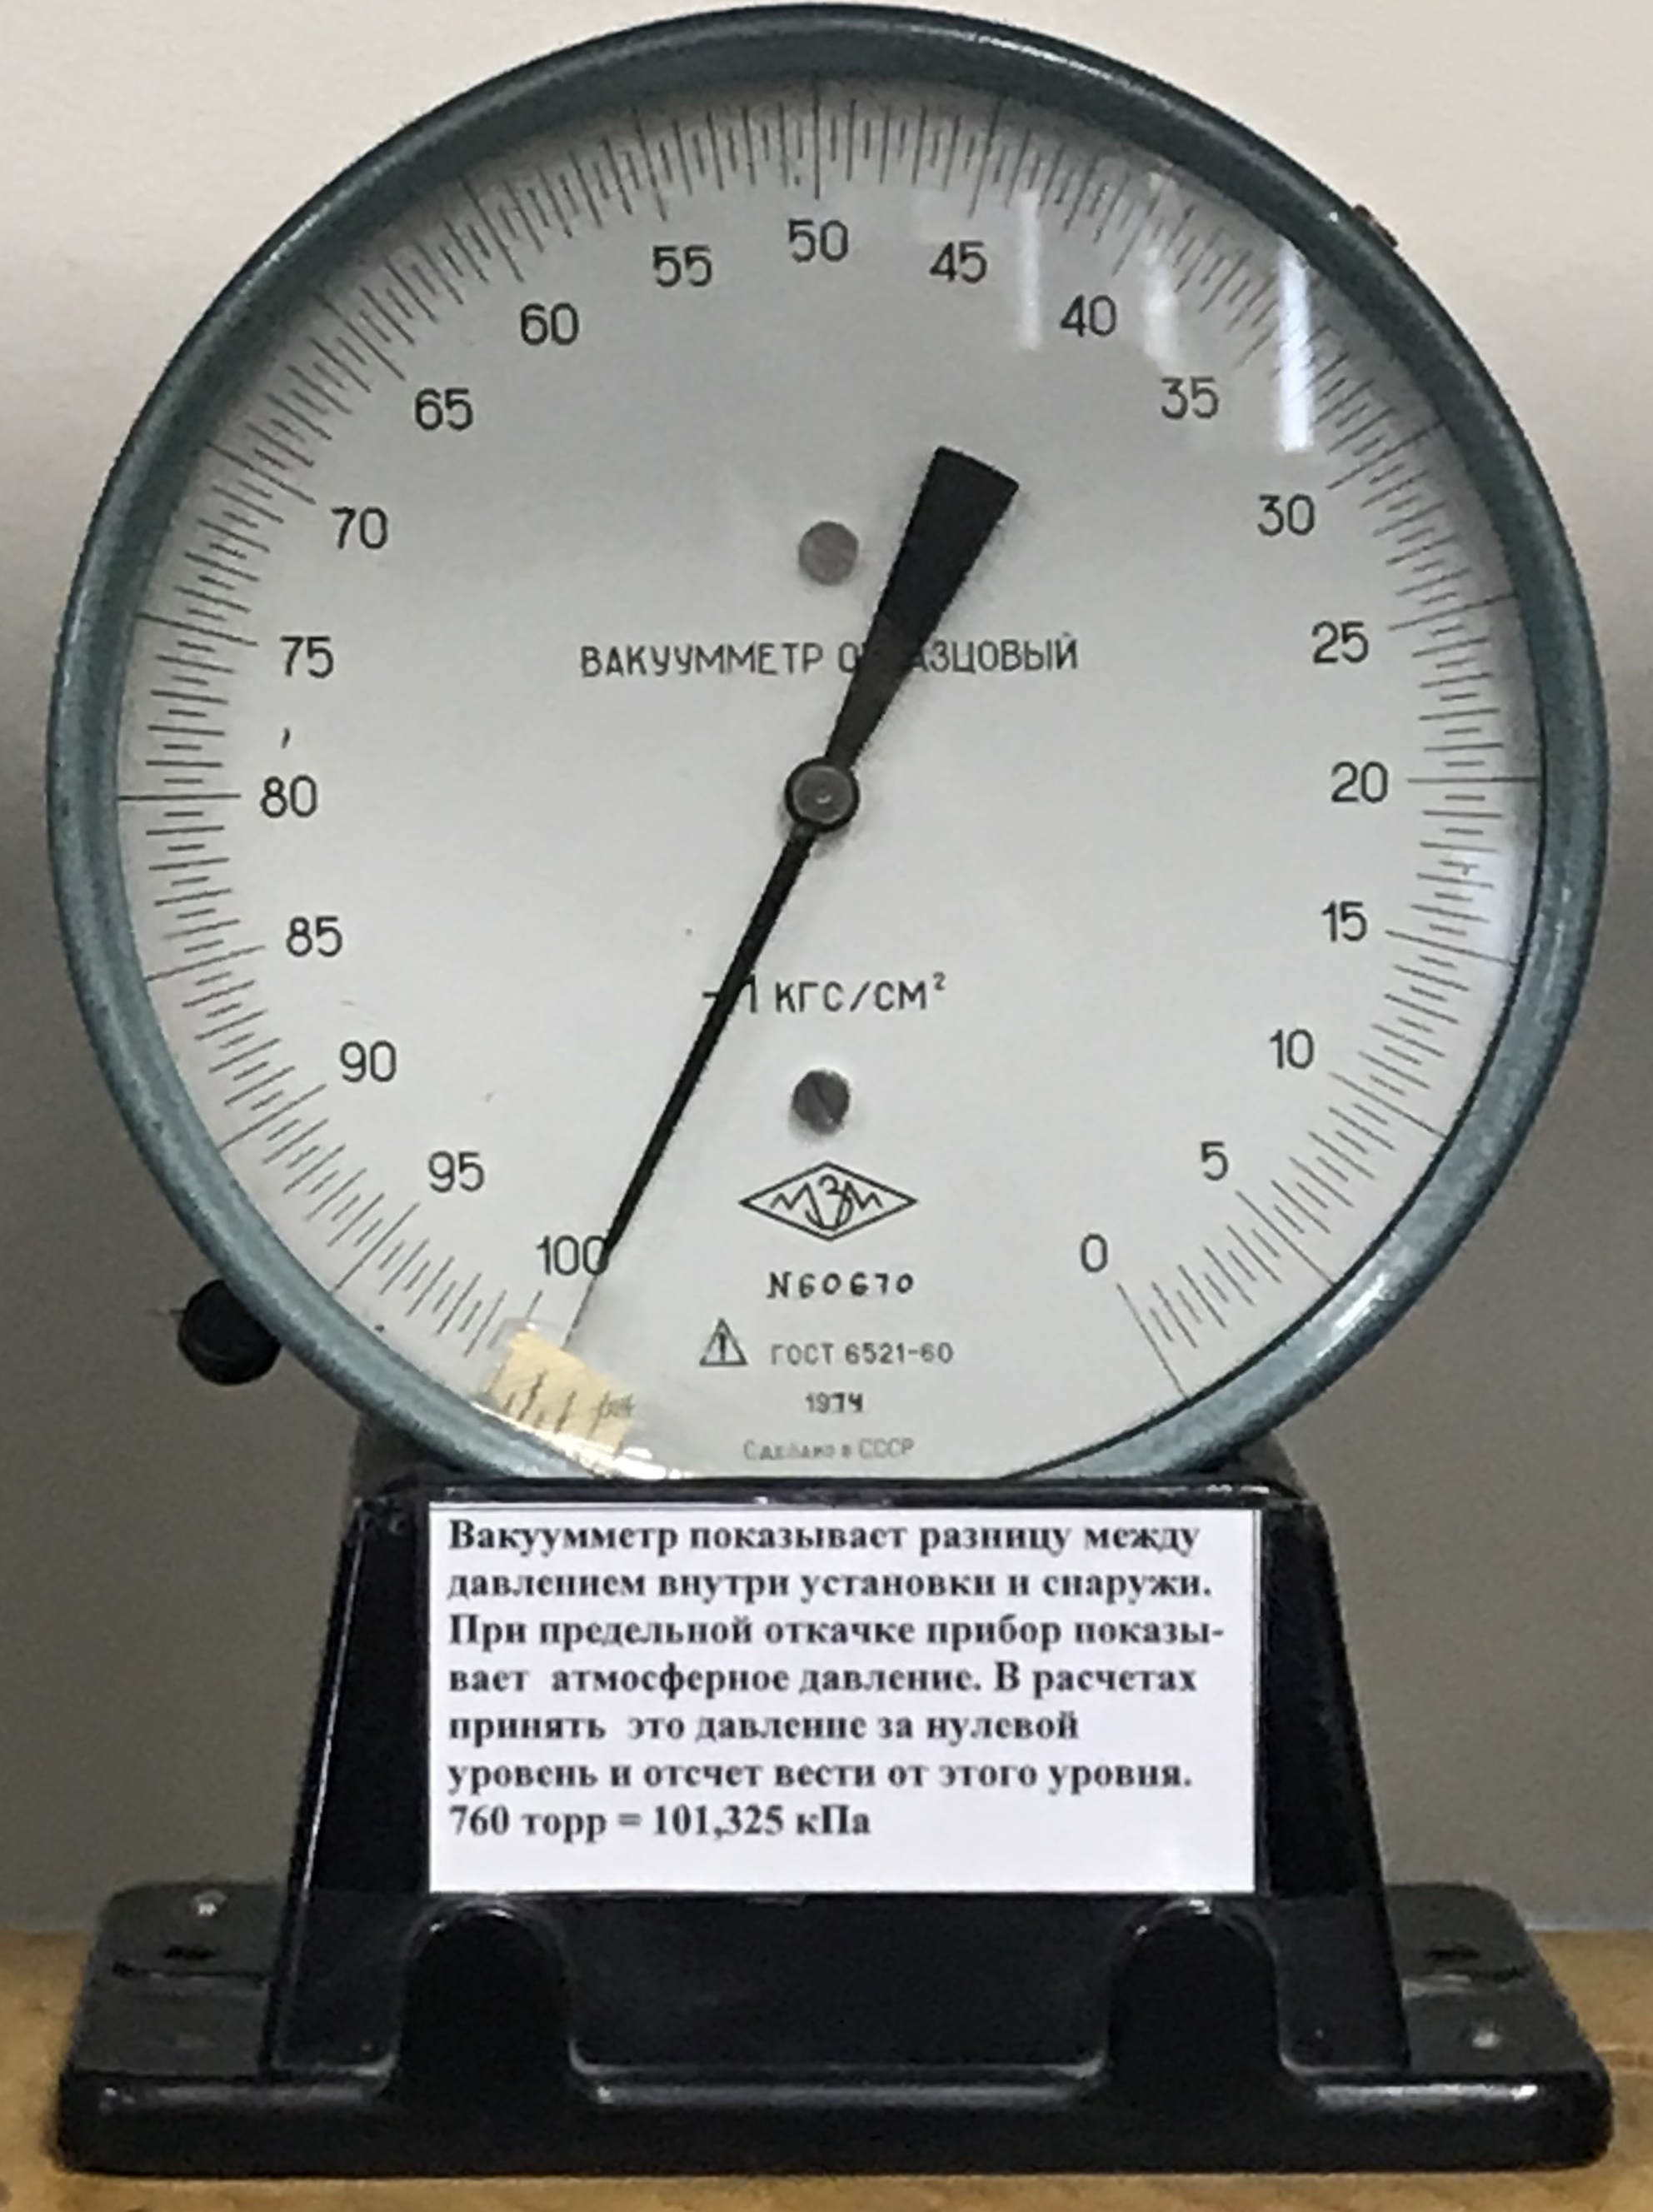
\includegraphics[scale=0.055]{vac.jpg} 
	\caption{Вакуумметр} 
\end{wrapfigure}

\subparagraph*{В работе используются:}измерительная установка (Рис. 3); форвакуумный насос; баллон с газом (гелий); манометр (Рис. 1); источник питания; магазин сопротивлений; гальванометр;  компьютерное ПО.

\subparagraph*{Теоретические сведения.} Диффузией называют самопроизвольное взаимное проникновение веществ друг в друга, происходящее вследствие хаотичного теплового движения молекул. При перемешивании молекул разного сорта говорят о взаимной (или концентрационной) диффузии.

Диффузия в системе, состоящей из двух компонентов $a$ и $b$ (бинарная смесь), подчиняется закону Фика: плотности потока компонентов  $j_{a, b}$ (количество частиц, пересекающих единичную площадку в единицу времени) пропорциональны градиентам их концентраций $\nabla n_{a, b}$, что в одномерном случае можно записать как
$$
j_a = -D\frac{\partial n_a}{\partial x}, j_b= -D\frac{\partial n_b}{\partial x}, 
$$
 где $D $ -- коэффициент взаимной диффузии компонентов. Знак "минус" отражает тот факт, что диффузия идёт в направлении выравнивания концентраций. Равновесие достигается при равномерном распределении вещества по объёму сосуда ( $\partial n / \partial x = 0$).
 
 В данной работе исследуется взаимная диффузия гелия и воздуха. Давление $P$ и температура $T$ в условиях опыта предполагаются неизменными: $P = (n_{He}+ n_в)k_БT=const$ ,где $n_{He}$ и $n_в$ -- концентрации (объёмные плотности) диффундирующих газов. Поэтому для любых изменений концентраций справедливо $\Delta n_{He} = - \Delta n_и$. Следовательно, достаточно ограничиться
 описанием диффузии одного из компонентов, например гелия $n_{He}$ :
 
 \begin{equation}\label{1}
j_{He}= -D\frac{\partial n_{He}}{\partial x}
 \end{equation}
 
 
  	\begin{wrapfigure}{l}{0.4\linewidth} 
 	\centering 
 	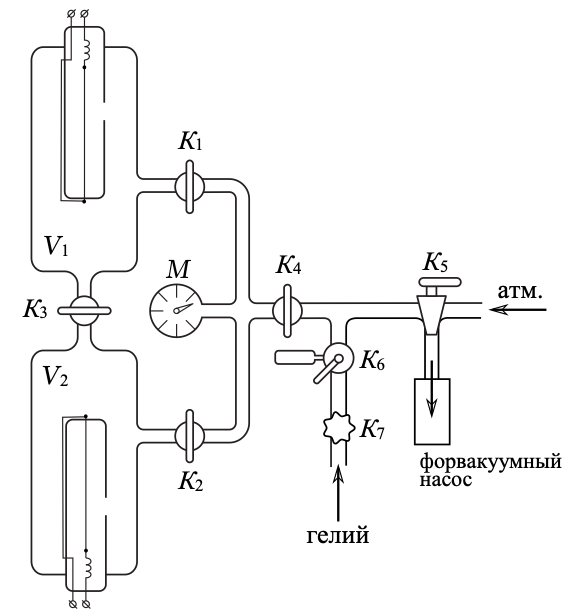
\includegraphics[scale=0.25]{1.jpg} 
 	\caption{Установка для исследования взаимной диффузии газов} 
 \end{wrapfigure}
 
 Приведём теоретическую оценку для коэффициента диффузии. В работе концентрация гелия, как правило, мала. Кроме того, атомы гелия существенно легче молекул, составляющих воздух ($\mu_{He} \ll \mu_{H_2}, \mu_{O_2}$), значит
 и их средняя тепловая скорость велика по сравнению с остальными частицами. Поэтому перемешивание газов в работе можно приближенно описывать как диффузию примеси лёгких частиц He на практически стационарном фоне воздуха. Коэффициент диффузии в таком приближении равен
 
 \begin{equation}\label{2}
 D = \frac{1}{3}\lambda\overline{v}, 
 \end{equation}
 где $\overline{v} = \sqrt{\frac{8RT}{\pi \mu}}$ -- средняя тепловая скорость частиц примеси, $\lambda = \frac{1}{n_0 \sigma}$ -- их длина свободного пробега, $n_0 $ -- концентрация рассеивающих центров (фона), $\sigma$ -- сечение столкновения частиц примеси с частицами фона. 
 
 
   	\begin{wrapfigure}{r}{0.45\linewidth} 
 	\centering 
 	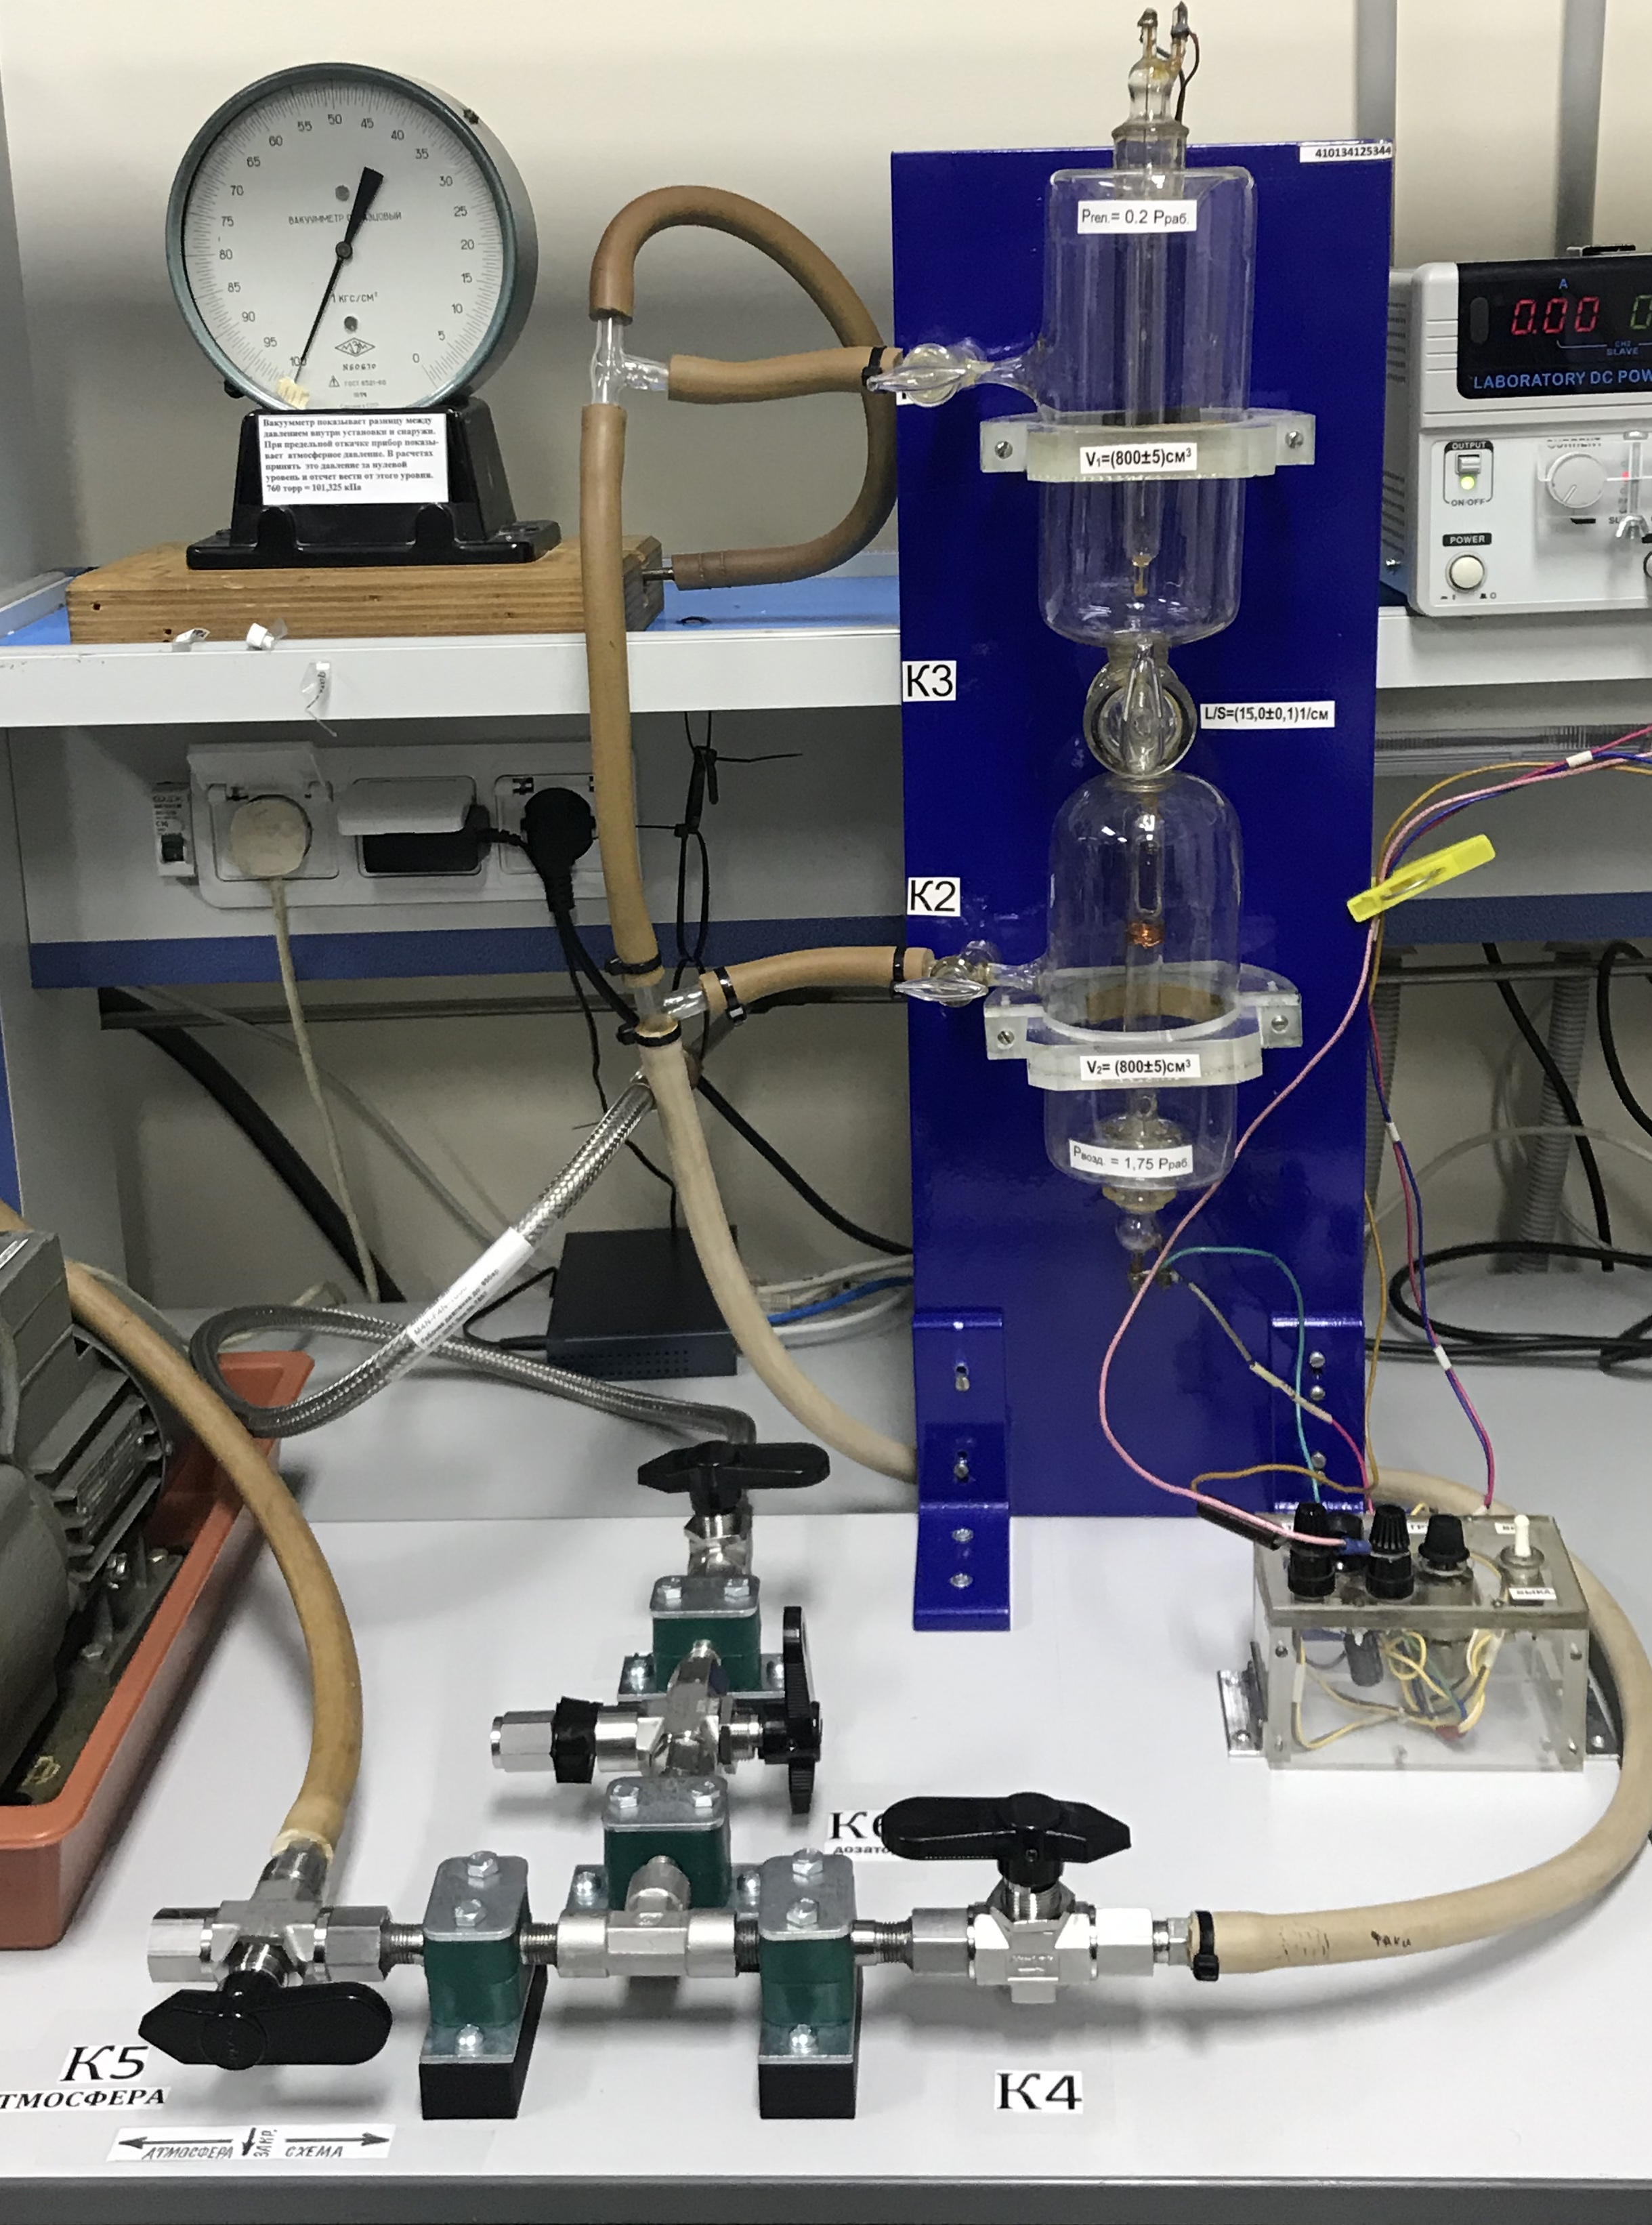
\includegraphics[scale=0.065]{plan.jpg} 
 	\caption{Внешний вид основной части установки} 
 \end{wrapfigure}

 
 Таким образом, теория показывает, что коэффициент диффузии обратно пропорционален давлению в системе и не зависит от пропорций компонентов, что и предлагается проверить в работе экспериментально. 
 

 
 
 \subparagraph*{Схема установки и методика измерения.} 
 
 Схема установки представлена на Рис.2. Краны $K_1$ и $K_2$ отвечают за изоляцию сосудов $V_1$ и $V_2$, а кран $K_3$ -- за сообщение между ними. Краны $K_6$ и  $K_7$ отвечают за подачу гелия. Гелий содержится в баллоне  под давлением, превышающим атмосферное. 

\subparagraph*{}Для предотвращения избыточного расхода гелия и его неконтролируемого проникания в установку предусмотрен металлический кран ($K_7$), отделяющий её от баллона с гелием. Его открывают только на время непосредственного заполнения установки гелием, остальное время он должен быть закрыт. 


\begin{wrapfigure}{r}{0.25\linewidth} 
	\centering 
	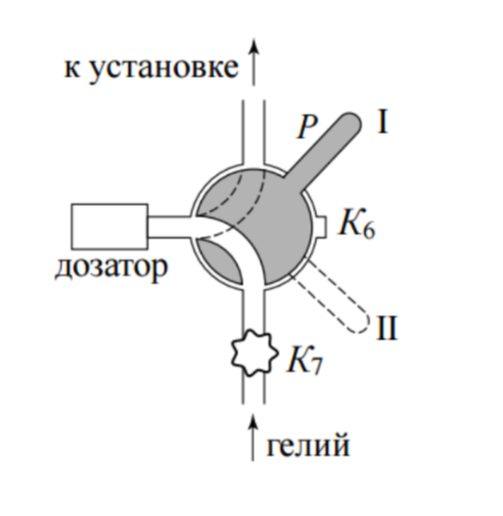
\includegraphics[scale=0.17]{3.jpg} 
	\caption{Кран $K_6$} 
\end{wrapfigure}

Для подачи малых порций гелия предусмотрен двухходовый кран с дозатором . При повороте рычажка $Р$ в положение I гелий в небольшом количестве поступает в дозатор (если открыт $K_7$),  а при повороте $Р$ в положение II порция из дозатора поступает в установку (схема работы представлена на Рис. 4). Кран $K_4$  обладает повышенной вакуумплотностью и используется для изоляции измерительной части установки от возможных протечек гелия и воздуха. Двухходовой кран $K_5$ служит для подключения форвакуумного насоса к установке, подачи воздуха в установку и соединения форвакуумного насоса с атмосферой. 

\begin{wrapfigure}{l}{0.25\linewidth} 
	\centering 
	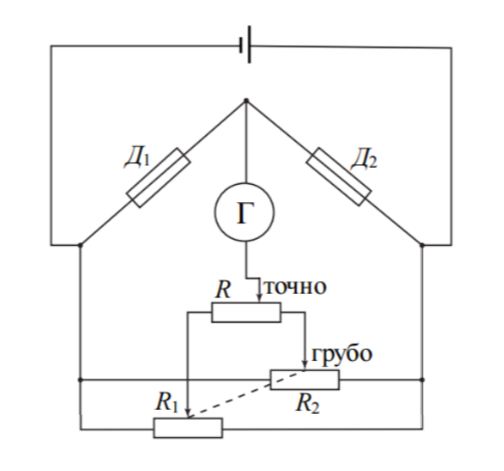
\includegraphics[scale=0.18]{2.jpg} 
	\caption{Схема работы банка сопротивлений} 
\end{wrapfigure}

Для измерения разности концентраций газов используется мостовая схема, представленная на Рис. 5. Здесь $D_1, D_2$ -- датчики теплопроводности, расположенные в сосудах $V_1$ и $V_2$. Сопротивления $R_1, R_2, R$ служат для установки прибора на нуль (балансировка моста). В одну из диагоналей моста включен гальванометр, к другой подключается небольшое постоянное напряжение. Сопротивления $R_1$ и $R_2$ спарены (их подвижные контакты находятся на общей оси) и изменяются одновременно при повороте ручки грубой регулировки. Точная балансировка выполняется потенциометром $R$. Балансировку необходимо проводить перед каждым экспериментом заново: при этом установка заполняется чистым газом (воздухом без гелия) при давлении, близком «рабочему» (при котором затем будут проводится измерения).

Мост балансируется при заполнении сосудов (и датчиков) одной и той же смесью. При заполнении сосудов смесями различного состава возникает «разбаланc» моста. При незначительном различии в составах смесей показания гальванометра, подсоединённого к диагонали моста, будут пропорциональны разности концентраций примеси: $U \propto \Delta \kappa \propto \Delta n$.
 	
 	
Рассмотрим процесс выравнивания концентрации. Пусть концентрации одного из компонентов смеси в сосудах $V_1$ и $V_2$ равны $n_1$ и
$n_2$. Плотность диффузионного потока любого компонента (т. е. количество вещества, проходящее в единицу времени через единичную поверхность) определяется законом Фика:
$$j=-D\frac{\partial n}{\partial x},$$ где $D$ — коэффициент взаимной диффузии газов, а $j$ - плотность потока частиц.

В нашем случае ввиду того что, а) объем соединительной трубки мал по сравнению с объемами сосудов, б) концентрацию газов внутри каждого сосуда можно считать постоянной по всему объему. Диффузионный поток в любом сечении трубки одинаков. Поэтому, $$J=-DS\frac{n_1-n_2}{l}.$$

Обозначим через $\Delta n_1$ и $\Delta n_2$ изменения концентрации в объемах
$V_1$ и $V_2$ за время $\Delta t$. Тогда $V_1 \Delta n_1$ равно изменению количества компонента в объеме $V_1$, а $V_2 \Delta n_2$ — изменению количества этого компонента в $V_2$. Из закона сохранения вещества следует, что $V_1n_1+V_2n_2 = const$, откуда $V_1 \Delta n_1 = -V_2\Delta n_2.$ Эти изменения происходят вследствие диффузии, поэтому: $$V_1\Delta n_1=-V_2\Delta n_2.$$

С другой стороны $V_1\Delta n_1=J\Delta t$ и $V_1\frac{dn_1}{dt}=-DS\frac{n_1-n_2}{l}.$ Аналогично $V_2\frac{dn_2}{dt}=DS\frac{n_1-n_2}{l}$

Тогда $$\frac{d(n_1-n_2)}{dt}=-\frac{n_1-n_2}{l} \frac{V_1+V_2}{V_1V_2}  $$

Проинтегрируем и получим, что $$n_1-n_2=(n_1-n_2)_0 e^{-t/\tau},$$ где $(n_1-
n_2)_0$ — разность концентраций в начальный момент времени, $$\tau=\frac{V_1V_2}{V_1+V_2}\frac{l}{SD} \approx \frac{1}{2V}\frac{l}{SD}$$

Для измерения концентраций в данной установке применяются датчики теплопроводности $Д_1$, $Д_2$ (см. рис. 1) используется зависимость теплопроводности газовой смеси от ее состава.
Для измерения разности концентраций газов используется мостовая схема (рис. 1). Здесь $Д_1$ и $Д_2$ — датчики теплопроводности, расположенные в сосудах $V_1$ и $V_2$. Сопротивления $R_1, R_2$ и $R$ служат для установки прибора на нуль (балансировка моста). В одну из диагоналей моста включен гальванометр, к другой подключается небольшое постоянное напряжение. Мост балансируется при заполнении сосудов (и датчиков) одной и той же смесью.

При заполнении сосудов смесями различного состава возникает «разбаланc» моста. При незначительном различии в составах смесей показания гальванометра, подсоединённого к диагонали моста, будут пропорциональны разности концентраций примеси. В процессе диффузии
разность концентраций убывает по экспоненте, и значит по тому же закону изменяются во времени показания гальванометра $$U=U_0 \exp(-t/\tau)$$

Эту зависимость нам и предстоит проверить на практике. 
 	

\newpage

\section*{Ход работы}

\subparagraph*{1.}Ознакомимся с устройством установки, внимательно исследуем механизмы подачи гелия, а так же правила работы с форвакуумным насосом. 

\subparagraph*{2.} Подготовим установку к работе, а именнно проверим все ли краны поставлены в нужное положение, нет ли нигде утечек. Далее включим питание датчиков и измерительного моста. После чего откачаем установку. 


\subparagraph*{3.}  Сбалансируем мост при начальном рабочем давлении давлении $P_1 = 40$ торр. (На Рис. 6 приведена фотография показаний вольтметра при сбалансированном мосте)


\begin{wrapfigure}{l}{0.55\linewidth} 
	\centering 
	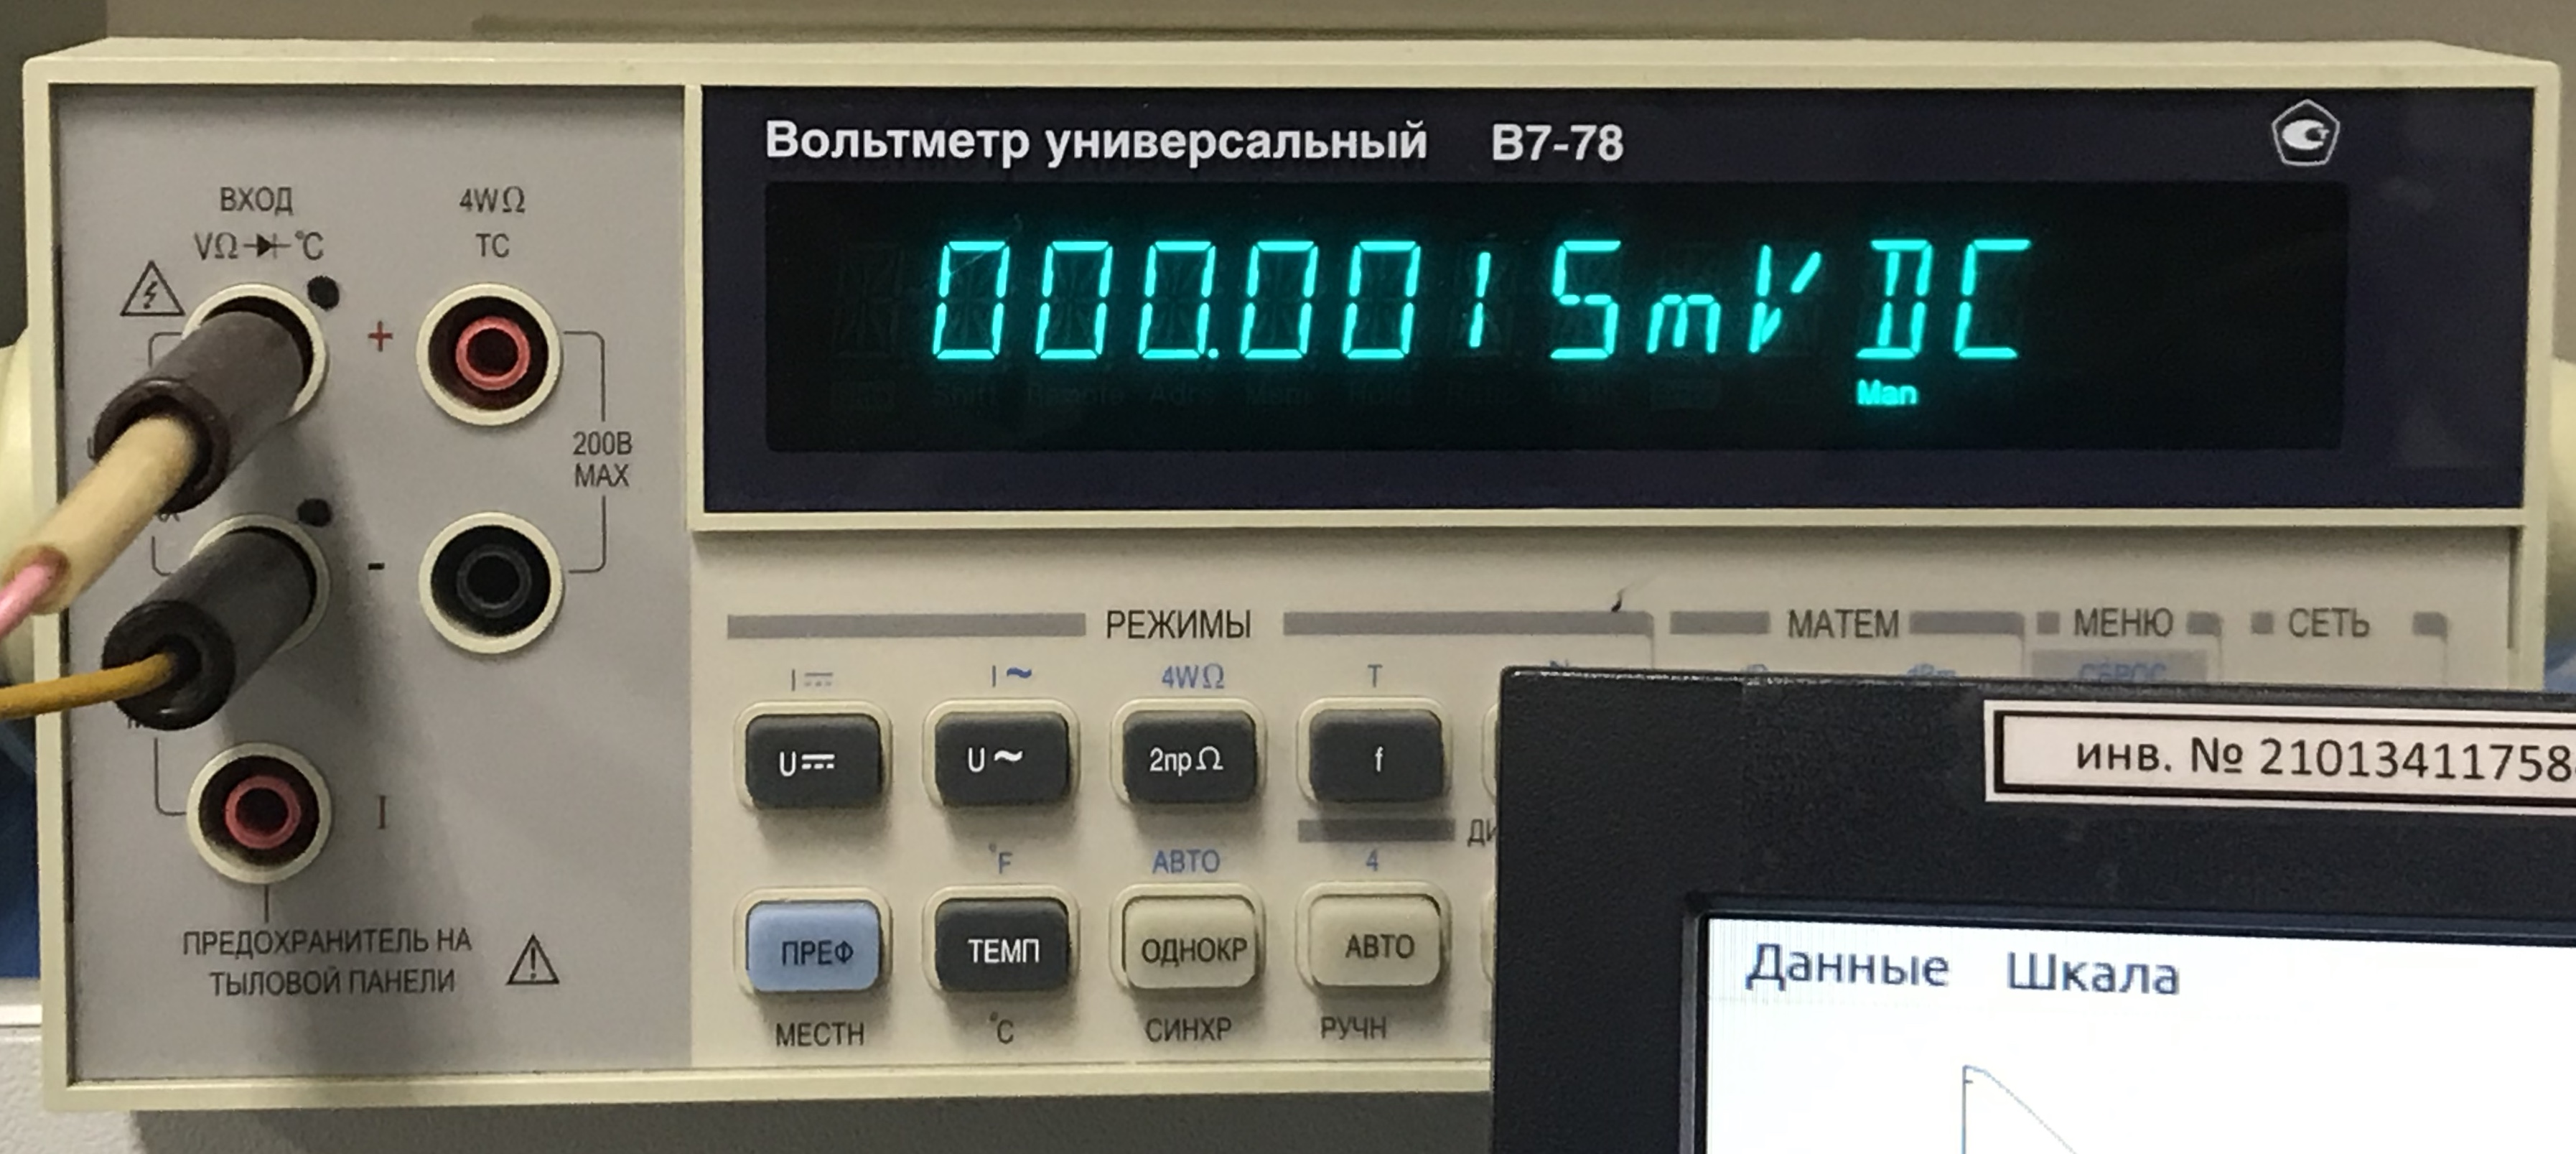
\includegraphics[scale=0.057]{br.jpg} 
	\caption{Вольтметр при сбалансированном мосте} 
\end{wrapfigure}


\subparagraph*{4.} Теперь нужно один из объёмов заполнить воздухом, а другой -- смесью гелия с воздухом. Сначала нужно заполнить объём, предназначенный для гелия, после чего нужно изолировать его и откачать гелий из патрубков. Затем заполнить второй объём воздухом.

\subparagraph*{} Следующим этапом необходимо уравнять давления в этих объёмах для чего нужно открыть краны $К_1$ и $К_2$ на небольшое время порядка 30 с, чтобы дать давлениям выравняться. После эти краны нужно перекрыть и записать давление, которое показывает манометр. 




\subparagraph*{5.} Откроем кран $К_3$, после чего начнётся процесс диффузии, перед этим необходимо запустить компьютерную программу, которая запишет показания вольтметра в зависимости от времени.  Из полученного массива данных выберем 15 точек для дальнейшего анализа и зафиксируем это в Таблице 1.



\subparagraph*{6.} Повторим измерения 3-5 для давлений до 240 торр.  Данные занесём в Таблицу 1.

\newpage

\section*{Обработка результатов эксперимента}

\subparagraph*{1.} Построим графики зависимости $\ln (U / U_0)$ от времени $t$ для выбранных точек. С помощью МНК вычислим коэффициент угла наклона для каждой прямой $k$ и погрешность этой величины.
$$k = \frac{\ln(U/U_0)}{t},$$
 $$\sigma_k = \frac{1}{\sqrt{n}}\sqrt{\frac{\left<\ln (U/U_0)^2\right>-\left<\ln (U/U_0)\right>^2}{\left<t^2\right>-\left<t\right>^2}-k^2}.$$ 
  Через эту величину выражается нужный нам коэффициент $D$ взаимной диффузии при заданном давлении, а именно $D = \frac{VL}{2\tau S}$, где $\tau = -\frac{t}{\ln (U/U_0)}=-\frac{1}{k}$ , то есть 
  $$D = -\frac{kVL}{2S},$$ 
  $$\sigma_D = D \sqrt{\big(\frac{\sigma_k}{k}\big)^2 + \big(\frac{3\sigma_V }{2V}\big)^2 + \big(\frac{\sigma_{L/S}}{L/S}\big)^2}.$$
  
  Для вычисления коэффициента взаимной диффузии $D$ нам нужны два параметра, которые записаны на установке, а именно:
  
  $  L/ S = (15.0 \pm 0.1) см^{-1}$ 
 
 
  $V = (800 \pm 5) см^3$
  
  
  Результаты представлены на Рис. 7 и в Таблице 1.
  
Как видно из Таблицы 1 относительная погрешность величины $k$, вносимая МНК, составляет не более 2\%, в то время как инструментальная погрешность составляет максимум (для оценки я взяла точки с максимальными относительными погрешностями) $\varepsilon_k = \varepsilon_t + \varepsilon_U \approx  0.03\% + 0.04\% \approx 0.1\%$, что гораздо меньше статистического вклада, поэтому инструментальнаю погрешность измерения величины $k$  в дальнейшем учитываться не будет. 





\subparagraph*{2.}


Построим график зависимости коэффициента диффузии от обратного давления и экстраполируя зависимость до атмосферного давления получим искомую величину коэффициента взаимной диффузии (обозначено зелёным  квадратом на Рис. 8). 
 \newpage


	\begin{table}[h!]
		\caption{Экспериментальные данные и их обработка}
		\begin{center}
			
			
			
			\begin{tabular}{||l|l|l||}
				\hline
				
				\multicolumn{3}{||l||}{\textbf{P = 41.3  торр}} \\ 
				\multicolumn{3}{||l||}{$1 / P = 1.82 \cdot 10^{-4}$ $Па^{-1}$} \\ \hline
				\multicolumn{3}{||l||}{$U_0 = 13.13$ mV} \\ \hline
				$U$, mV&$\ln (U/U_0)$ & $t$, s \\ \hline
				12.80 & -0.0256   &20.09 \\ \hline
				12.25 &  -0.0688 &40.09 \\ \hline
				11.73 & -0.112 &60.09  \\ \hline
				11.24 & -0.157 &80.09  \\ \hline
				10.77 & -0.197 &100.09  \\ \hline
				10.32  & -0.240 &120.09  \\ \hline
				9.90 & 	-0.282 &140.09  \\ \hline
				9.49 & -0.324&160.09  \\ \hline
				9.10 & -0.366 &180.09  \\ \hline
				8.73 & -0.408 &200.09  \\ \hline
				8.37 & -0.449  &220.09  \\ \hline
				8.03 & -0.490 &240.09  \\ \hline
				7.71 & -0.531 &60.09  \\ \hline
				7.41 & -0.572 &280.09  \\ \hline
				7.11 & -0.612  &300.09  \\ \hline
				6.83 &-0.653 & 320.09  \\ \hline
				6.56 & -0.692&340.09  \\ \hline
				6.31 &-0.732 & 360.09  \\ \hline
				6.07 & 	-0.771 &380.09  \\ \hline
				5.83  & -0.810 &400.09  \\ \hline
				\multicolumn{3}{||l||}{$k = -2.06 \cdot 10^{-3}$ s$^{-1}$} \\ 
				\multicolumn{3}{||l||}{$\sigma_k =0.1 \cdot 10^{-4}$ s$^{-1}$} \\ \hline 
				\multicolumn{3}{||l||}{$D = 12.40$ $cm^2/s$}\\ 
				\multicolumn{3}{||l||}{$\sigma_D =0.21$ $cm^2/s$} \\ \hline 
			\end{tabular}\begin{tabular}{||l|l|l||}
				\hline
				
				
				
				
				\multicolumn{3}{||l||}{\textbf{P = 77.5  торр}} \\ 
				\multicolumn{3}{||l||}{$1 / P = 9.68 \cdot 10^{-5}$ $Па^{-1}$} \\ \hline
				\multicolumn{3}{||l||}{$U_0 = 19.06$ mV} \\ \hline
				$U$, mV&$\ln (U/U_0)$ & $t$, s \\ \hline
				18.68 & -0.0199  &20.01 \\ \hline
				18.20 &  -0.0458 &40.01 \\ \hline
				17.73 & -0.0719&60.01  \\ \hline
				17.28 & -0.0975 &80.01  \\ \hline
				16.85 & -0.123 &100.01  \\ \hline
				16.42  & -0.148 &120.01  \\ \hline
				16.01& 	-0.174&140.01  \\ \hline
				15.61& -0.199&160.01  \\ \hline
				15.22& -0.224 &180.01  \\ \hline
				14.85& -0.249 &200.01  \\ \hline
				14.48& -0.274  &220.01  \\ \hline
				14.13& -0.298 &240.01 \\ \hline
				13.79& -0.323 &60.01\\ \hline
				13.45& -0.348 &280.01  \\ \hline
				13.13& -0.372  &300.01  \\ \hline
				12.81&-0.396& 320.01  \\ \hline
				12.51& -0.420&340.01  \\ \hline
				12.21&-0.444& 360.01  \\ \hline
				11.92& 	-0.468 &380.01  \\ \hline
				11.64& -0.492&400.01  \\ \hline
				\multicolumn{3}{||l||}{$k = -1.24\cdot 10^{-3}$ s$^{-1}$} \\ 
				\multicolumn{3}{||l||}{$\sigma_k =0.1 \cdot 10^{-4}$ s$^{-1}$} \\ \hline 
				\multicolumn{3}{||l||}{$D = 7.46 $ $cm^2/s$}\\ 
				\multicolumn{3}{||l||}{$\sigma_D =0.14$ $cm^2/s$} \\ \hline 
			\end{tabular}
			
			
			
			
		\end{center}
		
	\end{table}
	
	\newpage
	
	
	\begin{center}
		
		
		\begin{tabular}{||l|l|l||}
			\hline
			
			
			
			
			
			\multicolumn{3}{||l||}{\textbf{P = 120.4  торр}} \\ 
			\multicolumn{3}{||l||}{$1 / P = 6.23 \cdot 10^{-5}$ $Па^{-1}$} \\ \hline
			\multicolumn{3}{||l||}{$U_0 = 13.13$ mV} \\ \hline
			$U$, mV&$\ln (U/U_0)$ & $t$, s \\ \hline
			17.36& -0.0142 &20.09 \\ \hline
			17.05 &  -0.0325 &40.09 \\ \hline
			16.74 & -0.0510&60.09  \\ \hline
			16.43 & -0.0694&80.09  \\ \hline
			16.13 & -0.0877&100.09  \\ \hline
			15.85  & -0.105&120.09  \\ \hline
			15.57 & 	-0.123 &140.09  \\ \hline
			15.29 & -0.141&160.09  \\ \hline
			15.03& -0.158&180.09  \\ \hline
			14.77& -0.175 &200.09  \\ \hline
			14.52& -0.193  &220.09  \\ \hline
			14.27& -0.210 &240.09  \\ \hline
			14.03& -0.227 &60.09  \\ \hline
			13.79& -0.244 &280.09  \\ \hline
			13.56& -0.261  &300.09  \\ \hline
			13.34&-0.277& 320.09  \\ \hline
			13.11& -0.295&340.09  \\ \hline
			12.90&-0.311& 360.09  \\ \hline
			12.68& 	-0.328 &380.09  \\ \hline
			12.48& -0.344&400.09  \\ \hline
			\multicolumn{3}{||l||}{$k = -8.68 \cdot 10^{-4}$ s$^{-1}$} \\ 
			\multicolumn{3}{||l||}{$\sigma_k =0.6 \cdot 10^{-5}$ s$^{-1}$} \\ \hline 
			\multicolumn{3}{||l||}{$D = 5.21$ $cm^2/s$}\\ 
			\multicolumn{3}{||l||}{$\sigma_D =0.10$ $cm^2/s$} \\ \hline 	\end{tabular}\begin{tabular}{||l|l|l||}
			\hline
			
			
			
			
			\multicolumn{3}{||l||}{\textbf{P = 140.0  торр}} \\ 
			\multicolumn{3}{||l||}{$1 / P = 4.69 \cdot 10^{-5}$ $Па^{-1}$} \\ \hline
			\multicolumn{3}{||l||}{$U_0 = 19.06$ mV} \\ \hline
			$U$, mV&$\ln (U/U_0)$ & $t$, s \\ \hline
			16.71 & -0.0108  &20.01 \\ \hline
			16.48 &  -0.0249 &40.01 \\ \hline
			16.24 & -0.0393&60.01  \\ \hline
			16.01 & -0.0536 &80.01  \\ \hline
			15.79 & -0.0678&100.01  \\ \hline
			15.57  & -0.0818&120.01  \\ \hline
			15.36& 	-0.0955&140.01  \\ \hline
			15.15& -0.109&160.01  \\ \hline
			14.94& -0.122 &180.01  \\ \hline
			14.74& -0.136 &200.01  \\ \hline
			14.54& -0.149  &220.01  \\ \hline
			14.35& -0.163 &240.01 \\ \hline
			13.16& -0.176 &60.01\\ \hline
			13.98& -0.189 &280.01  \\ \hline
			13.80& -0.202  &300.01  \\ \hline
			13.62&-0.215& 320.01  \\ \hline
			13.45& -0.228&340.01  \\ \hline
			13.28&-0.240& 360.01  \\ \hline
			13.11& 	-0.253 &380.01  \\ \hline
			12.95& -0.266&400.01  \\ \hline
			\multicolumn{3}{||l||}{$k = -6.71\cdot 10^{-4}$ s$^{-1}$} \\ 
			\multicolumn{3}{||l||}{$\sigma_k =0.5 \cdot 10^{-5}$ s$^{-1}$} \\ \hline 
			\multicolumn{3}{||l||}{$D = 4.03$ $cm^2/s$}\\ 
			\multicolumn{3}{||l||}{$\sigma_D =0.08$ $cm^2/s$} \\ \hline 
		\end{tabular}
		
		
		
		
	\end{center}
	
	
	\newpage
	
	\begin{center}
		
		
		\begin{tabular}{||l|l|l||}
			\hline
			
			
			
			\multicolumn{3}{||l||}{\textbf{P = 200.0  торр}} \\ 
			\multicolumn{3}{||l||}{$1 / P = 3.75\cdot 10^{-5}$ $Па^{-1}$} \\ \hline
			\multicolumn{3}{||l||}{$U_0 = 19.06$ mV} \\ \hline
			$U$, mV&$\ln (U/U_0)$ & $t$, s \\ \hline
			16.95& -0.0113 &20.01 \\ \hline
			16.74 &  -0.0239 &40.01 \\ \hline
			16.53 & -0.0366&60.01  \\ \hline
			16.32 & -0.0495 &80.01  \\ \hline
			16.11 & -0.0620&100.01  \\ \hline
			15.91  & -0.0749&120.01  \\ \hline
			15.71& 	-0.0873&140.01  \\ \hline
			15.52& -0.0995&160.01  \\ \hline
			15.33& -0.111 &180.01  \\ \hline
			15.15& -0.123 &200.01  \\ \hline
			14.98& -0.135  &220.01  \\ \hline
			14.80& -0.147 &240.01 \\ \hline
			14.63& -0.158 &60.01\\ \hline
			14.47& -0.169 &280.01  \\ \hline
			14.30& -0.181  &300.01  \\ \hline
			14.15&-0.192& 320.01  \\ \hline
			13.99& -0.203&340.01  \\ \hline
			13.84&-0.214& 360.01  \\ \hline
			13.68& 	-0.225 &380.01  \\ \hline
			13.53& -0.237&400.01  \\ \hline
			\multicolumn{3}{||l||}{$k = -5.92\cdot 10^{-4}$ s$^{-1}$} \\ 
			\multicolumn{3}{||l||}{$\sigma_k =0.5 \cdot 10^{-5}$ s$^{-1}$} \\ \hline 
			\multicolumn{3}{||l||}{$D = 3.55$ $cm^2/s$}\\ 
			\multicolumn{3}{||l||}{$\sigma_D =0.08$ $cm^2/s$} \\ \hline 
		\end{tabular}\begin{tabular}{||l|l|l||}
			\hline
			
			
			\multicolumn{3}{||l||}{\textbf{P = 236.3  торр}} \\ 
			\multicolumn{3}{||l||}{$1 / P = 3.17\cdot 10^{-5}$ $Па^{-1}$} \\ \hline
			\multicolumn{3}{||l||}{$U_0 = 13.13$ mV} \\ \hline
			$U$, mV&$\ln (U/U_0)$ & $t$, s \\ \hline
			17.05 & -0.00796  &20.09 \\ \hline
			16.89 &  -0.0176&40.09 \\ \hline
			16.71 & -0.0280&60.09  \\ \hline
			16.54 & -0.0384 &80.09  \\ \hline
			16.37 & -0.0485 &100.09  \\ \hline
			16.21  & -0.0586 &120.09  \\ \hline
			16.05& 	-0.0687&140.09  \\ \hline
			15.89& -0.0784&160.09  \\ \hline
			15.74& -0.0878 &180.09  \\ \hline
			15.59& -0.0972&200.09  \\ \hline
			15.45& -0.106&220.09  \\ \hline
			15.30& -0.116 &240.09  \\ \hline
			15.16& -0.125 &60.09  \\ \hline
			15.02& -0.134 &280.09  \\ \hline
			14.88& -0.143  &300.09  \\ \hline
			14.75&-0.152& 320.09  \\ \hline
			14.61& -0.162&340.09  \\ \hline
			14.48&-0.171& 360.09  \\ \hline
			14.35& 	-0.180 &380.09  \\ \hline
			14.23& -0.189&400.09  \\ \hline
			\multicolumn{3}{||l||}{$k = -4.76 \cdot 10^{-4}$ s$^{-1}$} \\ 
			\multicolumn{3}{||l||}{$\sigma_k =0.6\cdot 10^{-5}$ s$^{-1}$} \\ \hline 
			\multicolumn{3}{||l||}{$D = 2.86$ $cm^2/s$}\\ 
			\multicolumn{3}{||l||}{$\sigma_D =0.07$ $cm^2/s$} \\ \hline 
		\end{tabular}
		
		
		
		
	\end{center}

\newpage

\begin{figure}[h!]
	\centering 
	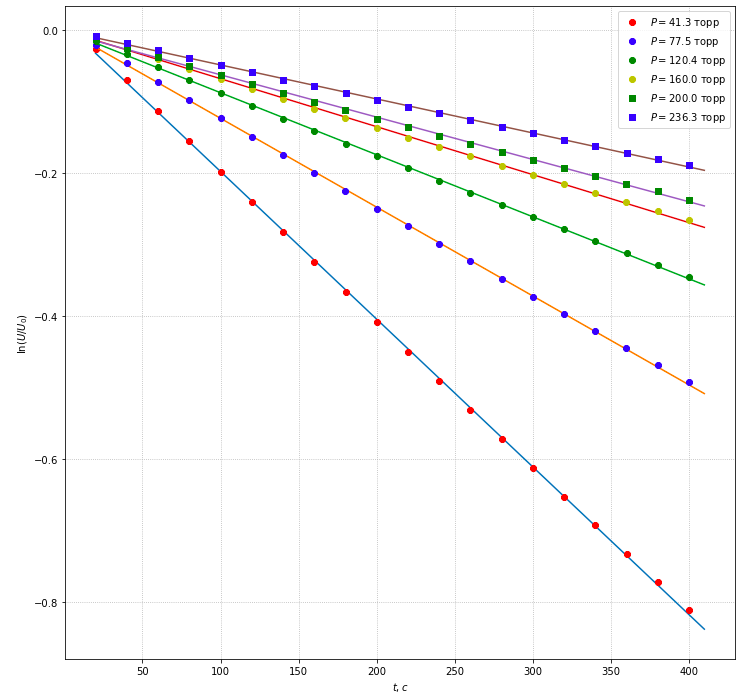
\includegraphics[scale=0.5]{g1.jpg} 
	\caption{График зависимости  $\ln (U / U_0)$ от времени $t$ } 
\end{figure}



\begin{figure}[h!]
	\centering 
	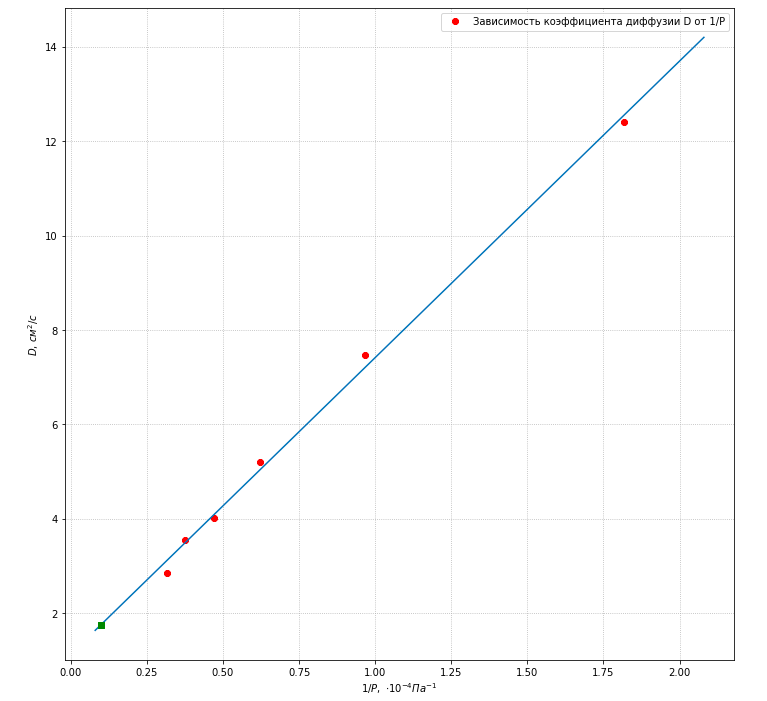
\includegraphics[scale=0.5]{g3.jpg} 
	\caption{График зависимости  $D$ от обратного давления $1/P$ } 
\end{figure}


Точность измерения давления определяется инструментальной погрешностью используемого вакуумметра и составляет порядка $6\%$ (значение для маленьких двалений 20-40 торр). Используя МНК получим, что погрешность полученного значения ещё $7\%$, то есть в результате погрешность величины $\varepsilon_{D_{атм} }= 10\%$

Поэтому итоговый ответ $D_{атм} = (1.76 \pm 0.18)$ $ cm^2/s$, что даже в пределах погрешности не стыкуется с табличным значением 0.66 $ cm^2/s$, хоть и имеет с ним один порядок.

\newpage

\subparagraph*{3.}


Теперь по полученным данным оценим длину свободного пробега и размер молекулы.  Поскольку 
$D = \frac{1}{3} \lambda \langle v \rangle,\;$ где $\langle v \rangle = \sqrt{\frac{8RT}{\pi \mu}},$
то длина свободного пробега $\lambda = 3D\sqrt{\dfrac{\pi \mu}{8RT}} \approx 420$ нм, что сходится с табличными значениями только по порядку.


Эффективное сечение  $\sigma = \dfrac{kT}{\sqrt{\lambda P}} \approx 6.9 \cdot 10^{-2} $ $нм^2$.



	
\newpage
	
\section*{Вывод}

В ходе работы мо научились работать с форвакуумным насосом, а так же с вакуумным оборудованием. Убедились в том, что во время диффузии для концентраций газов выполняется соотношение  $\Delta n = \Delta n_0 e^{-\frac{t}{\tau}}$. Так же мы проверили, что коэффициент взаимной диффузии $D$ линейно зависит от обратного давления $1 / P$, при этом экстраполируя значения давления к атмосферному мы смогли получить приближенной значение $D_{атм}$. Полученное значение сходится с табличным по порядку. Так же используя величину $D_{атм}$ мы смогли получить оценки для длины свободного пробега атомов гелия $\lambda$ и  эффективного сечения столкновения в смеси воздух-гелий $\sigma_{He-воздух}$. 


\end{document}
